This chapter goes more in depth of the specifics on the experiments conducted. It describes the exact hardware specifications and software libraries used. It also defines all the different experiments and includes several figures for added information. At first the hardware used will be discussed. After that the software and it's specifications. Finally every experiment that is conducted and their definitions.
\section{Hardware}
The hardware used for this experiment are specially designed clusters made with Raspberry Pi's 3 model B+. These Pi's are assigned using the same ratio of FLPs and EPNs at CERN (1:6) and 1 Information Node. The Pi's are modified with an extra Ethernet port. The exact specifications are in table ~\ref{table:RaspberrySpecifications}.

\begin{table}[htb]
\begin{tabular}{| l | l |}
\hline
Processor & Cortex-A53 1.4GHZ\\ \hline
RAM & 1GB LPDDR2 SDRAM\\ \hline
Network & 1 300MbE 1 10/100MbE \\ \hline
Operating System & Raspbian Stretch (Debian 9)\\ \hline
\end{tabular}
\caption{Specifications modified Raspberry Pi 3 model B+}
\label{table:RaspberrySpecifications}
\end{table}

~\\ Everything is setup and built from a single server unit. The IP addresses are also managed from this unit. Specifications are in table ~\ref{table:ManagementSpecifications}.

\begin{table}[htb]
\begin{tabular}{| l | l |}
\hline
Processor & Cortex-A53 1.4GHZ\\ \hline
RAM & 1GB LPDDR2 SDRAM\\ \hline
Network & 300MbE\\ \hline
Operating System & Raspbian Stretch (Debian 9)\\ \hline
\end{tabular}
\caption{Specifications management server}
\label{table:ManagementSpecifications}
\end{table}

\newpage

~\\ The network configuration consists of a bidirectional connection. This is used to reduce the bottleneck over one interface. Load Balancing is done over the first interface, and monitoring is done over the second interface. Figure ~\ref{fig:NetworkSetup} shows a network overview:
\begin{figure}[htb]
    \centering
    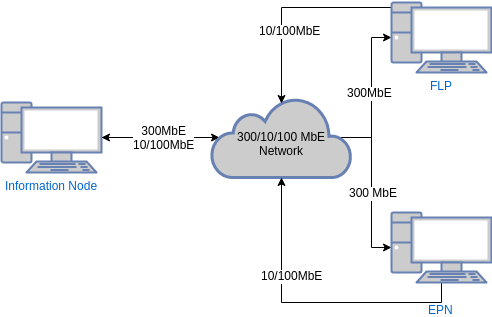
\includegraphics[scale=0.5]{./graphics/Network_thesis.png}
    \caption{Network setup}
    \label{fig:NetworkSetup}
\end{figure}

~\\ The clusters of Pi's are build using sets of four Raspberry Pi 3 Model B+ with extra ethernet interfaces. These are connected to each other using two tp-link TL-SF100D switches. From these switches the sets of Pi's are connected through one Juniper EX3400 Ethernet switch. Specifications are in table ~\ref{table:EthernetSpeeds}. This setup is used because of the high amount of ethernet ports required, and a switch that could accomidate all of it (+/- 60) was not available.

\begin{table}[htb]
\begin{tabular}{| l | l |}
\hline
Switch & Speed \\ \hline
tp-link TL-SF100D & 10/100Mbps \\ \hline
Juniper EX3400 & 1/10GbE \\
\hline
\end{tabular}
\caption{Ethernet switch speeds}
\label{table:EthernetSpeeds}
\end{table}

\subsection{Complications}
The second interface is obtained using a LogiLink UA0025C USB2.0 to Ethernet adapter. This adapter has a speed of 10MbE/100MbE and is primarily used by Zookeeper to register which Pi is still running. During the build of the prototype there was also an option of using an ENC28J60 Ethernet board instead. This would be plugged onto the GPIO pins on the Raspberry Pi. This board is a lot slower than the LogiLink though, clocking in at around 380 KB/s. 

\begin{figure}[htb]
	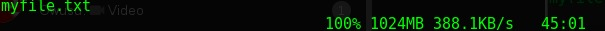
\includegraphics[width=\textwidth]{./graphics/gpio_ethernet_speed.jpg}
	\caption{ENC28J60 Ethernet board connection speed}
\end{figure}

~\\ At first the experiments were done using one set of four Pi's using the ENC28J60 boards, and three sets of four Pi's using the LogiLink adapter. During these experiments it was found out that the ENC28J60 boards weren't that reliable. The FLPs and Information Node were using these interfaces, but during tests they would completely disable and ruin the tests results. After that an experiment was done by swapping the FLPs and Information Node with EPNs. This result showed that the specific EPNs would disable midway through as well. Because of this the one set of Pi's was also converted to use the LogiLink instead.

\section{Software}
The software used is found at https://github.com/SoftwareForScience/O2-Balancer. It consists of 3 executable programs to represent a FLP, EPN and Information Node. These programs are sent to the devices to represent their respective units. Apart from that it uses a stripped down version of FairRoot (FairRootGroup/FairRoot, 2018). Since only the FairMQ (FairRootGroup/FairMQ, 2018) part is needed for the programs to run it has been split off from this code.\\
The Infomation Node serves two purposes. At first it generates the TFs that are send to the FLPs using FairMQ. It also receives notifications from the EPNs when they have received the full TF from the FLPs again. The configuration is done using YAML files. A diagram of the connections and dependencies are shown in figure ~\ref{fig:SoftwareFigure} and table ~\ref{table:SoftwareDependencies}.

\begin{figure}[htb]
    \centering
    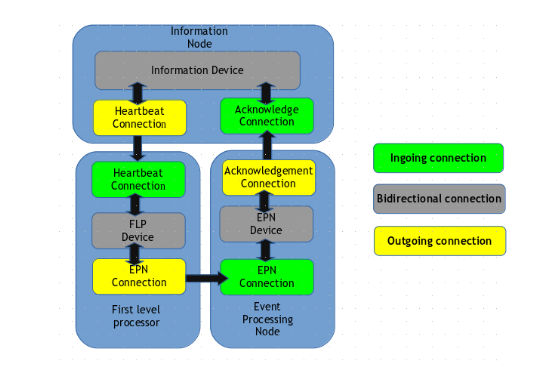
\includegraphics[scale=0.7]{./graphics/connection_diagram.png}
    \caption{Block diagram of the cluster connections (van der Heijden, 2018, p. 22)}
    \label{fig:SoftwareFigure}
\end{figure}

\begin{table}[htb]
\begin{tabular}{| l | l |}
\hline
Library/Tool & Version \\ \hline
FairMQ & 1.1.5\\ \hline
ZeroMQ & 4.2.1\\ \hline
Zookeeper & 3.4.9 \\ \hline
Cmake & 3.11.0 \\ \hline
Boost & 1.66.0 \\ \hline
Yaml-cpp & 0.5.2 \\ \hline
Compiler & gcc 6.3.0 20170516 (Raspbian 6.3.0-18+rpi1+deb9u1)\\ \hline
\end{tabular}
\caption{Dependencies software}
\label{table:SoftwareDependencies}
\end{table}

\newpage
\newpage

\section{Data analysis tools}
In order to stay consistent with the previous experiment, the same tools will be used to create and visualize the data. This can be found at \\ https://github.com/valvy/BalancerScripts. These scripts are written in Python and ROOT to generate graphs and histograms from the log files received from the software. The dependencies are specified in table ~\ref{table:AnalysisDependencies}.

\begin{table}[ht]
\begin{tabular}{| l | l |}
\hline
Tool & Version \\ \hline
Operating system & Centos 7 \\ \hline
ROOT & 6.13.02 \\ \hline
Python & 2.7.13 \\ \hline
Ansible & 2.2.1 \\ \hline
Scipy & 1.1.0 \\ \hline
\end{tabular}
\caption{Dependencies for the analysis scripts}
\label{table:AnalysisDependencies}
\end{table}

\newpage

\section{Experiments}
In order to check whether or not the Information Node has any issues with increased numbers of FLPs and EPNs, the same experiments need to be done as described in the previous report (van der Heijden, 2018, p23-p27) but will be briefly summarized again. The experiments are done in two steps. At first the experiments need to be run using the same amount of FLPs and EPNs to verify whether or not the new setup of Raspberry Pi clusters are able to give the same result. After that the experiments need to be run again using more FLPs and EPNs to check if it indeed does have an effect on the Information Node. Lastly two additional experiments will be conducted to check whether or not the layout of the system architecture is of influence to the TF loss.

\subsection{Experiment one}
\textbf{Ticktime influence on the Blacklist algorithm with one fail-over.}
\\~\\
The first experiment uses a fixed sample size to be sent from the Information Node, and will have 1 fail-over during its run. This sample size is set to 100 kilobyte and the heartbeat rate is set to twenty milliseconds. This heartbeat is set at the same rate used at CERN. This sample size is set to accommodate the slower Ethernet and processing speed of Raspberry Pi as compared to units used in the previous experiment (van der Heijden, 2018, p.23). \\
This experiment will disable one EPN when it receives the first STF from hearbeat 3.000. Then special scripts will parse the logfiles between heartbeat 2.000 and 10.000 to have enough of a buffer to read from. A flowchart is shown in figure ~\ref{fig:FlowChart1}.

\begin{figure}
    \centering
    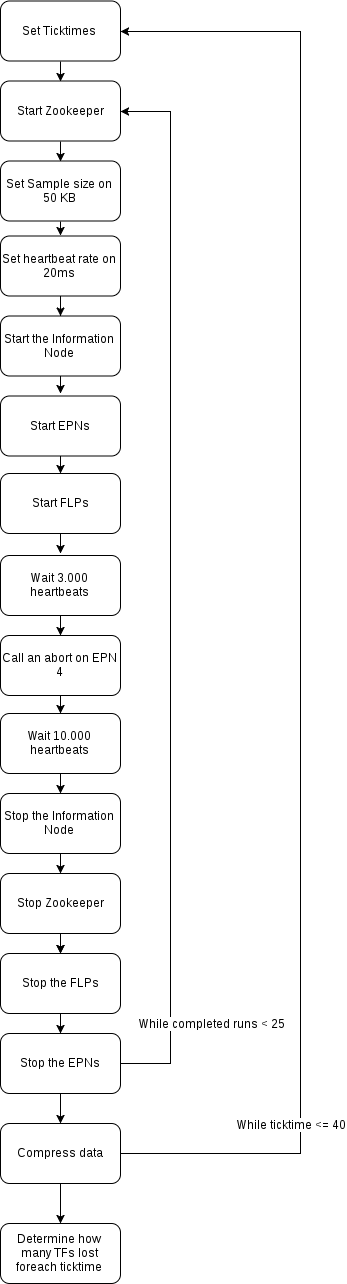
\includegraphics[width=\textwidth,height=\textheight,keepaspectratio]{./graphics/ex1.png}
    \caption{Flow chart experiment one}
    \label{fig:FlowChart1}
\end{figure}

\newpage
\subsection{Experiment two}
\textbf{Ticktime influence on the Blacklist algorithm with all but one fail-over.}
\\~\\
The same heartbeat rate and sample size are used from experiment one. For this experiment the first EPN will be disabled at heartbeat 2.000. After that every 1.000 heartbeats an additional EPN will be disabled until there is only 1 left. Scripts will parse all the logs to check how many TFs were lost during this progress. A flowchart can be found in figure ~\ref{fig:FlowChart2}.

\begin{figure}[htb]
    \centering
    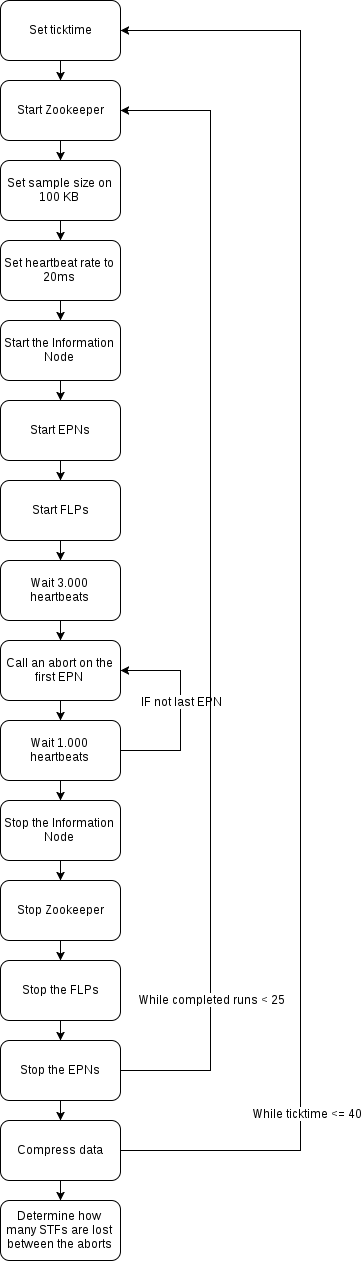
\includegraphics[width=\textwidth,height=\textheight,keepaspectratio]{./graphics/ex2.png}
    \caption{Flow chart experiment two}
    \label{fig:FlowChart2}
\end{figure}

\subsection{Experiment three}
\textbf{Ticktime influence on the Blacklist algorithm with all but one fail-over with random sample size.}
\\~\\
The same heartbeat rate is used from experiment one. A random sample size will be generated from the FLPs with an average size of 100 kilobytes. Apart from that the same configuration will be used as in experiment two. The first EPN will be disabled at heartbeat 2.000 and after that every 1.000 heartbeats an additional EPN will be disabled. A flowchart can be found in figure ~\ref{fig:FlowChart3}.

\begin{figure}[htb]
    \centering
    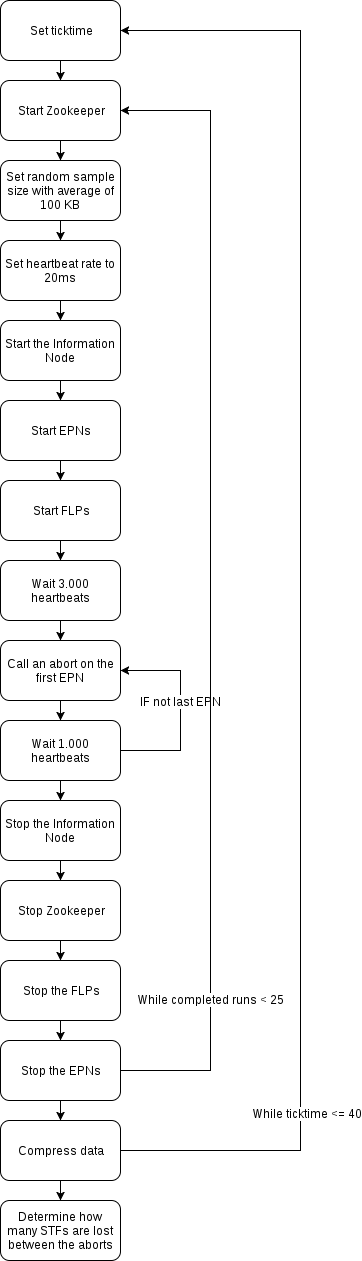
\includegraphics[width=\textwidth,height=\textheight,keepaspectratio]{./graphics/ex3.png}
    \caption{Flow chart experiment three}
    \label{fig:FlowChart3}
\end{figure}

\subsection{Experiment four}
\textbf{Ticktime influence on the Blacklist algorithm with a fixed cluster fail-over pattern using a random sample size}
\\~\\
The same heartbeat rate is used from experiment one. The same random sample size from experiment three is used. For this experiment the first cluster of four raspberry pi's will be disabled at heartbeat 3.000. After that every 2.000 heartbeats an additional cluster will be disabled until there is only one cluster left. A flowchart can be found in figure ~\ref{fig:FlowChart4}.

\begin{figure}[htb]
	\centering
	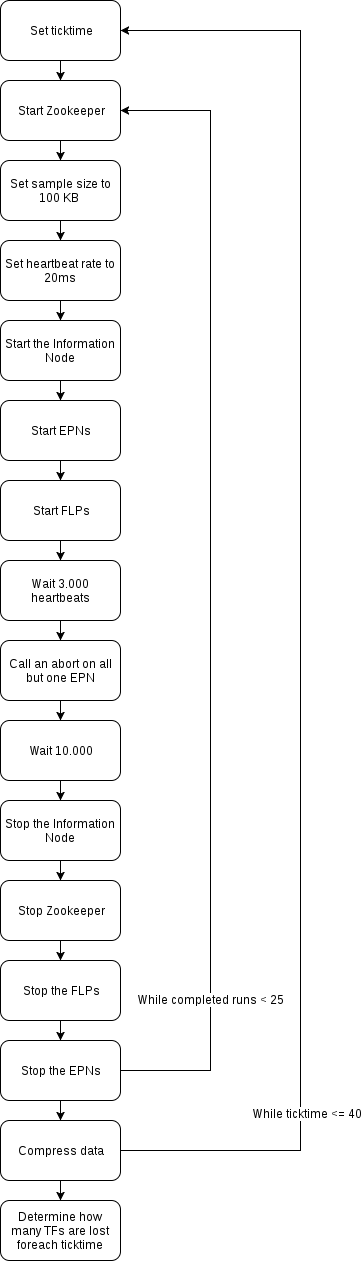
\includegraphics[width=\textwidth,height=\textheight,keepaspectratio]{./graphics/ex4.png}
	\caption{Flow chart experiment four}
	\label{fig:FlowChart4}
\end{figure}

\subsection{Experiment five}
\textbf{Ticktime influence on the Blacklist algorithm with a random cluster fail-over pattern using a random sample size}
\\~\\
The same heartbeat rate is used from experiment one. The same random sample size from experiment three will be used. For this experiment a random set of four raspberry pi's will be disabled at heartbeat 3.000. After that, every 2.000 heartbeats an additional set of four pi's are disabled until there is only one set left. A flowchart can be found in figure ~\ref{fig:FlowChart5}.

\begin{figure}[htb]
	\centering
	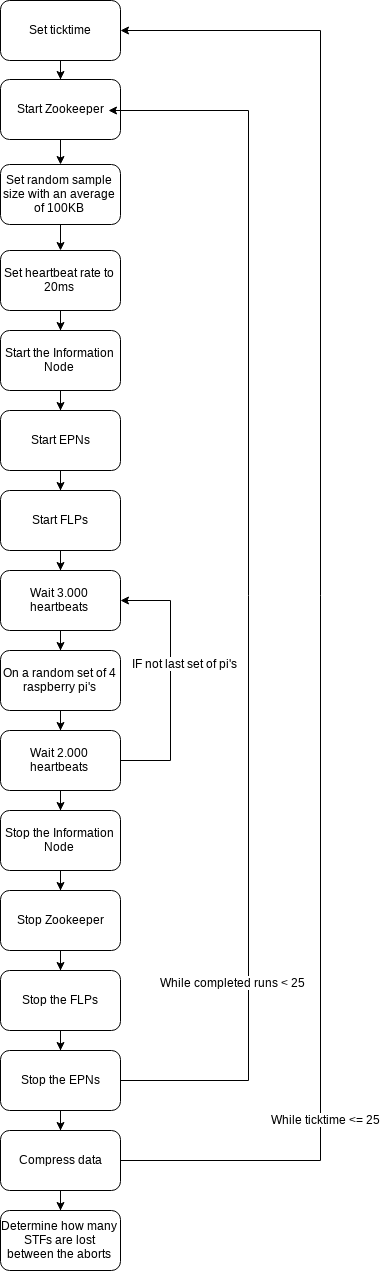
\includegraphics[width=\textwidth,height=\textheight,keepaspectratio]{./graphics/ex5.png}
	\caption{Flow chart experiment five}
	\label{fig:FlowChart5}
\end{figure}